\section{Results and Discussion}

Euclidian coordinates performed better when speaking of efficiency in terms of accuracy and speed. 76.92\% of the Euclidian charts shown resulted in the a correct identification of the real data while only 20.31\% of the polar charts did the same. A t-test comparing means for charts with polar coordinates versus charts with Euclidian coordinates resulted in a t statistic of 15.2013 with a p-value of 2.2e-16. Similarly, a t-test comparing means of time spent on charts with Euclidian coordinates versus charts with polar coordinates resulted in a p-value of 1.014e-11. The average of the log of time spent on each individual chart for charts with Euclidian coordinates is 3.53 minutes while it was 4.07 minutes for charts with polar coordinates. Euclidian coordinates resulted in a significantly more accurate identification of the real data set in significantly shorter time. 

\begin{figure}[htbp] %  figure placement: here, top, bottom, or page
   \centering
   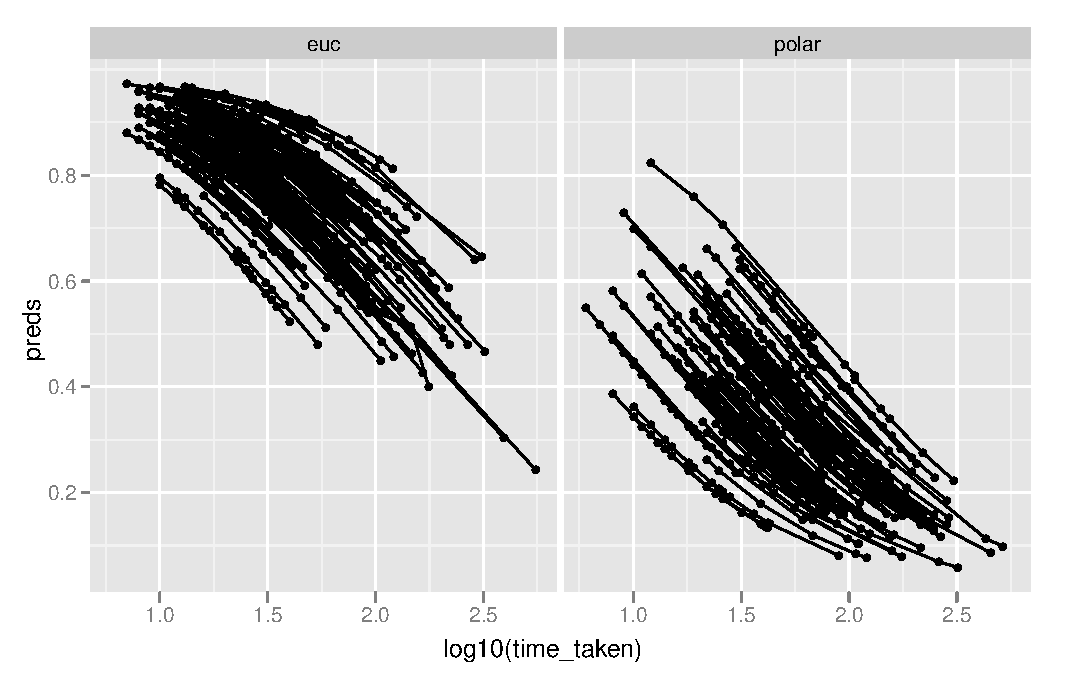
\includegraphics[width=3in]{turk4_time_perc_preds.pdf}  
   \caption{Values predicted from XXXX how to say itXXXX of accuracy for log of time taken and test parameter.}
   \label{accuracy_preds}
\end{figure}

Figure \ref{accuracy_preds} shows predicted accuracy levels. These predicted values were obtained by using R package lme4 and a mixed effect model explaining correct responses by type of chart and the log of time spent while accounting for different levels of accuracy for each individual who participated in the experiment. The predicted values show that there is an overall higher accuracy level for Euclidian coordinates when compared to polar coordinates. For both chart types, as the time spent increases, the predicted accuracy decreases. 



